\documentclass[tikz]{standalone}
\usepackage{pgfplots}
\usepackage{xcolor} % Needed for hex colors
\usetikzlibrary{calc} % For coordinate calculations if needed
\definecolor{markcolor}{HTML}{3c78d8} % Define the custom color
\pgfplotsset{compat=1.18}

\begin{document}
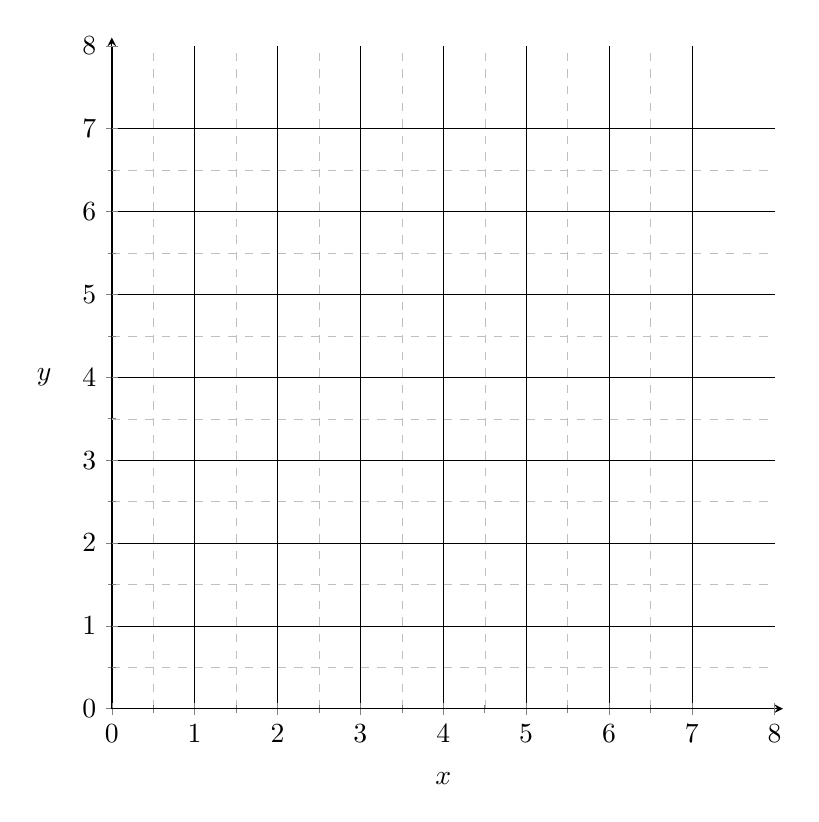
\begin{tikzpicture}
  \begin{axis}[
    % Draw only the bottom and left axes with arrow tips:
    axis lines=left,
    x axis line style={->,>=stealth, shorten >=-3pt},
    y axis line style={->,>=stealth, shorten >=-3pt},
    xlabel={$x$},
    ylabel={$y$},
    % Rotate the y label so that it appears upside down:
    ylabel style={rotate=-90},
    xmin=0, xmax=8,
    ymin=0, ymax=8,
    % Major ticks (and grid lines) at integers 0 through 7:
    xtick={0,1,...,7},
    ytick={0,1,...,7},
    % Extra ticks at 8 (no grid lines):
    extra x ticks={8},
    extra x tick style={grid=none},
    extra y ticks={8},
    extra y tick style={grid=none},
    % Place one minor tick between each major tick (i.e. at 0.5 steps):
    minor x tick num=1,
    minor y tick num=1,
    grid=both,
    % Grid styling:
    major grid style={line width=0.2pt,draw=black},
    minor grid style={line width=0.1pt,draw=gray!50,dashed},
    width=10cm,
    height=10cm,
  ]
    % Add a filled circle marker at (3,6) with the specified color:
    \addplot[only marks, mark=circle*, mark options={scale=1.5, fill=markcolor}] coordinates {(3,6)};
  \end{axis}
\end{tikzpicture}
\end{document}